

%\begin{frame}{Reference 2 s}
%	\cite{yang2023diffusestylegesture}
%\end{frame}


%\begin{frame}[allowframebreaks]{References}
%	{\footnotesize
%    \printbibliography}
%\end{frame}


%\appendix
%
%\section{Phụ lục}
%
%\begin{frame}{Ký hiệu}
%	\textbf{Tham số}: Đang huấn luyện {\Large$\textcolor{cyan}{\theta}$}, đã huấn luyện xong: {\Large$\textcolor{cyan}{\theta}'$}, {\Large$\textcolor{cyan}{\hat{\bx}}$}: dự đoán
%	\vspace{-5pt}
%	
%	\textbf{Phân phối chuẩn}
%	\vspace{-5pt}
%	{\Large $$\mathcal{N}(\textcolor{red}{a} \mathbf{x}, \textcolor{blue}{b^2})$$}
%	\vspace{-15pt}
%	\begin{itemize}
%		\item Một hàm $f(x) = a x + b\epsilon$ với $\epsilon \in \mathcal{N}(0, \mathbf{1})$ được ký hiệu là $f(x) \sim \mathcal{N}(a x, b^2) $
%		
%		\item Trung bình: $\mu = \textcolor{red}{a}x=\frac{1}{n} \sum_{i=1}^{n} x_i$
%		
%		\item Phương sai: $\sigma^2 = \textcolor{blue} {b^2} = \frac{1}{n} \sum_{i=1}^{n} (x_i - \mu)^2$
%		
%	\end{itemize}
%	\textbf{xác suất có điều kiện}
%	\vspace{-5pt}
%	{\Large $$p(\textcolor{green}{x}| \textcolor{orange}{y})$$}
%	\vspace{-15pt}
%	
%	\begin{itemize}
%		\item $p(\textcolor{green}{x}| \textcolor{orange}{y})$ là xác suất có điều kiện.
%		\item $\textcolor{orange}{y}$: xảy ra trước (bên phải)
%		\item $\textcolor{green}{x}$: sảy ra sau y (bên trái)
%	\end{itemize}
%	
%\end{frame}

%
%\begin{frame}
%	%	Mỗi Bone được biểu diễn thành: 
%	%	$$q = w + xi + yj + zk$$
%	%	
%	%	$$i^2 = j^2 = k^2 = ijk = -1$$
%	\begin{figure}
%		\centering
%		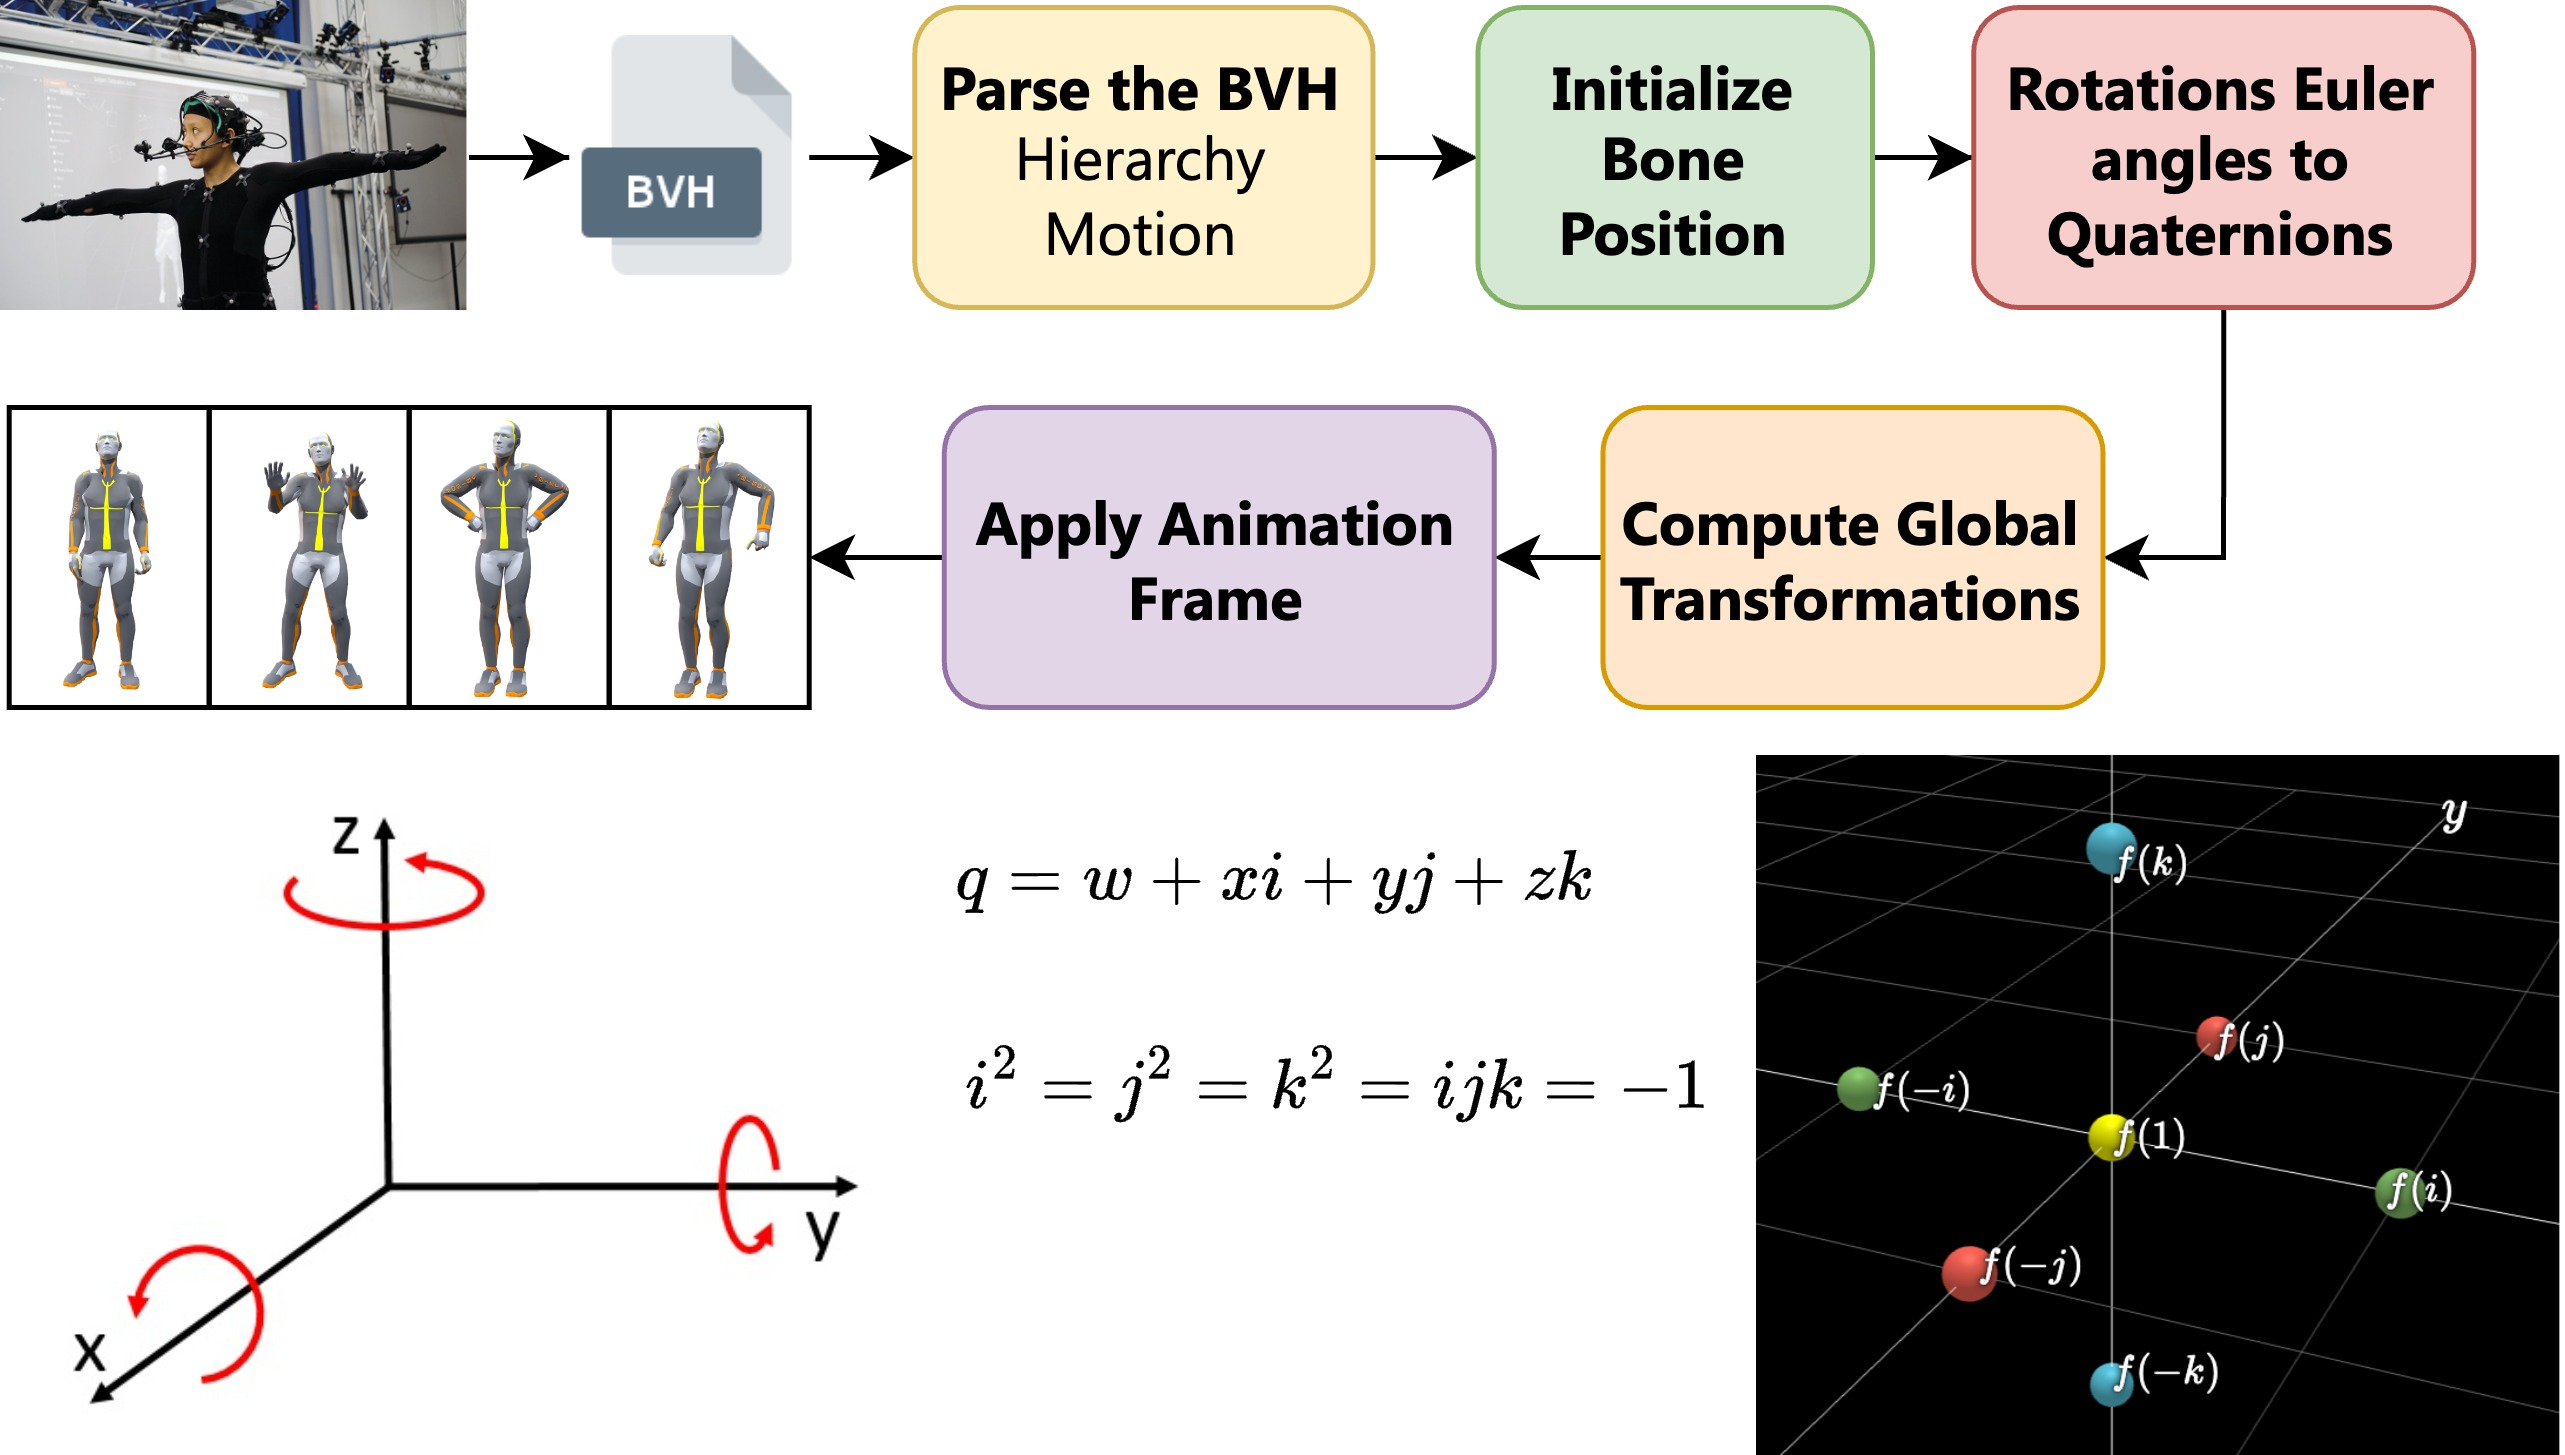
\includegraphics[width=\textwidth]{BVH}
%	\end{figure}
%\end{frame}
%
%
%\begin{frame}{Góc quay của một khung xương}
%	\small
%	\textbf{Hierachy}: bao gồm 75 Bone $\{ \mathbf{t}_i \}^{75} $, có vị trí ban đầu  $\mathbf{t}_{i} = \{t_x, t_y, t_z\}$
%	
%	\vspace{5pt}
%	
%	\textbf{Bone} trong dữ liệu BVH bao gồm vị trí $\mathbf{position}_{\operatorname{local}}  \in \mathbb{R}^{3}$ và góc quay $\mathbf{rotation}_{\operatorname{local}} \in \mathbb{R}^{3}$.
%	%	\begin{figure}
%		%		\centering
%		%		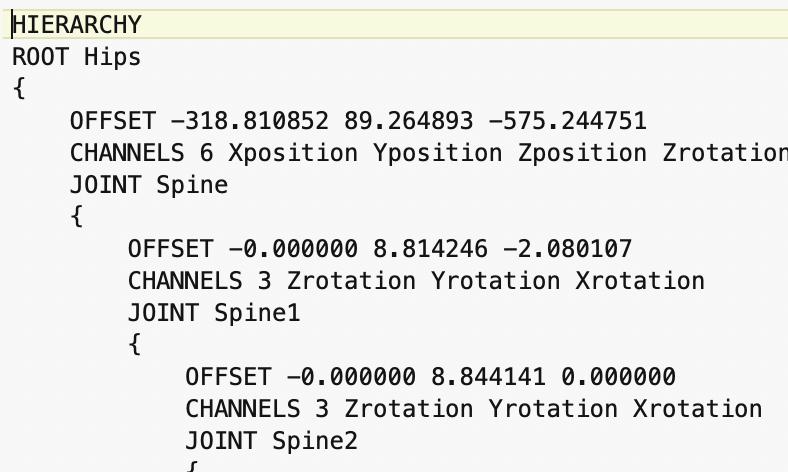
\includegraphics[width=0.25\textwidth]{BVHFile}
%		%	\end{figure}
%	$\mathbf{rotation}_i^{\operatorname{local}} = \{ \alpha ,\beta , \gamma \}$ lần lượt là góc quay quanh các trục $Z$ ,$Y$ , và $X$, góc quay tổng hợp trong không gian Eule là $R = R_Z(\alpha) R_Y(\beta) R_X(\gamma)$:
%	\begin{equation}
%		\mathbf{position}_{\text{global}} = R \cdot \mathbf{position}_{\text{local}} + \mathbf{t}
%	\end{equation}
%	Chuyển góc quay từng Bone dạng Euler ZYX sang dạng Quaternion, mỗi Bone biểu diễn bằng $q = (q_w, q_x, q_y, q_z)$
%	%	Mỗi Bone được biểu diễn thành: 
%	%	$$q = w + xi + yj + zk$$
%	%	c
%	%	$$i^2 = j^2 = k^2 = ijk = -1$$
%	\begin{columns}
%		\begin{column}{0.5\textwidth}
%			\begin{itemize}
%				\item $c_{\alpha} = \cos\left(\frac{\alpha}{2}\right), \quad s_{\alpha} = \sin\left(\frac{\alpha}{2}\right)$
%				\item $c_{\beta} = \cos\left(\frac{\beta}{2}\right), \quad s_{\beta} = \sin\left(\frac{\beta}{2}\right)$
%				\item $c_{\gamma} = \cos\left(\frac{\gamma}{2}\right), \quad s_{\gamma} = \sin\left(\frac{\gamma}{2}\right)$
%			\end{itemize}
%		\end{column}
%		\begin{column}{0.5\textwidth}
%			\begin{itemize}
%				\item $q_w = c_{\alpha} c_{\beta} c_{\gamma} + s_{\alpha} s_{\beta} s_{\gamma}$
%				\item $q_x = c_{\alpha} c_{\beta} s_{\gamma} - s_{\alpha} s_{\beta} c_{\gamma}$
%				\item $q_y = c_{\alpha} s_{\beta} c_{\gamma} + s_{\alpha} c_{\beta} s_{\gamma}$
%				\item $q_z = s_{\alpha} c_{\beta} c_{\gamma} - c_{\alpha} s_{\beta} s_{\gamma}$
%			\end{itemize}
%		\end{column}
%	\end{columns}
%	\begin{equation}
%		\mathbf{p}_{\text{global}} = q \cdot \mathbf{p}_{\text{local}} \cdot q^{-1} + \mathbf{t}
%	\end{equation}
%	
%	$\mathbf{t}$ là vị trí gốc của bone trong không gian toàn cục.
%\end{frame}
%
%
%
%
%\begin{frame}{$q(\bx_t | \bx_{t-1})$ và $p_{\theta}(\bx_{t-1} | \bx_t ) $  trong DDPM }
%	\textbf{DDPM} (Denoising Diffusion Probabilistic Model \cite{ho2020denoisingdiffusionprobabilisticmodels})
%	\begin{figure}
%		\centering
%		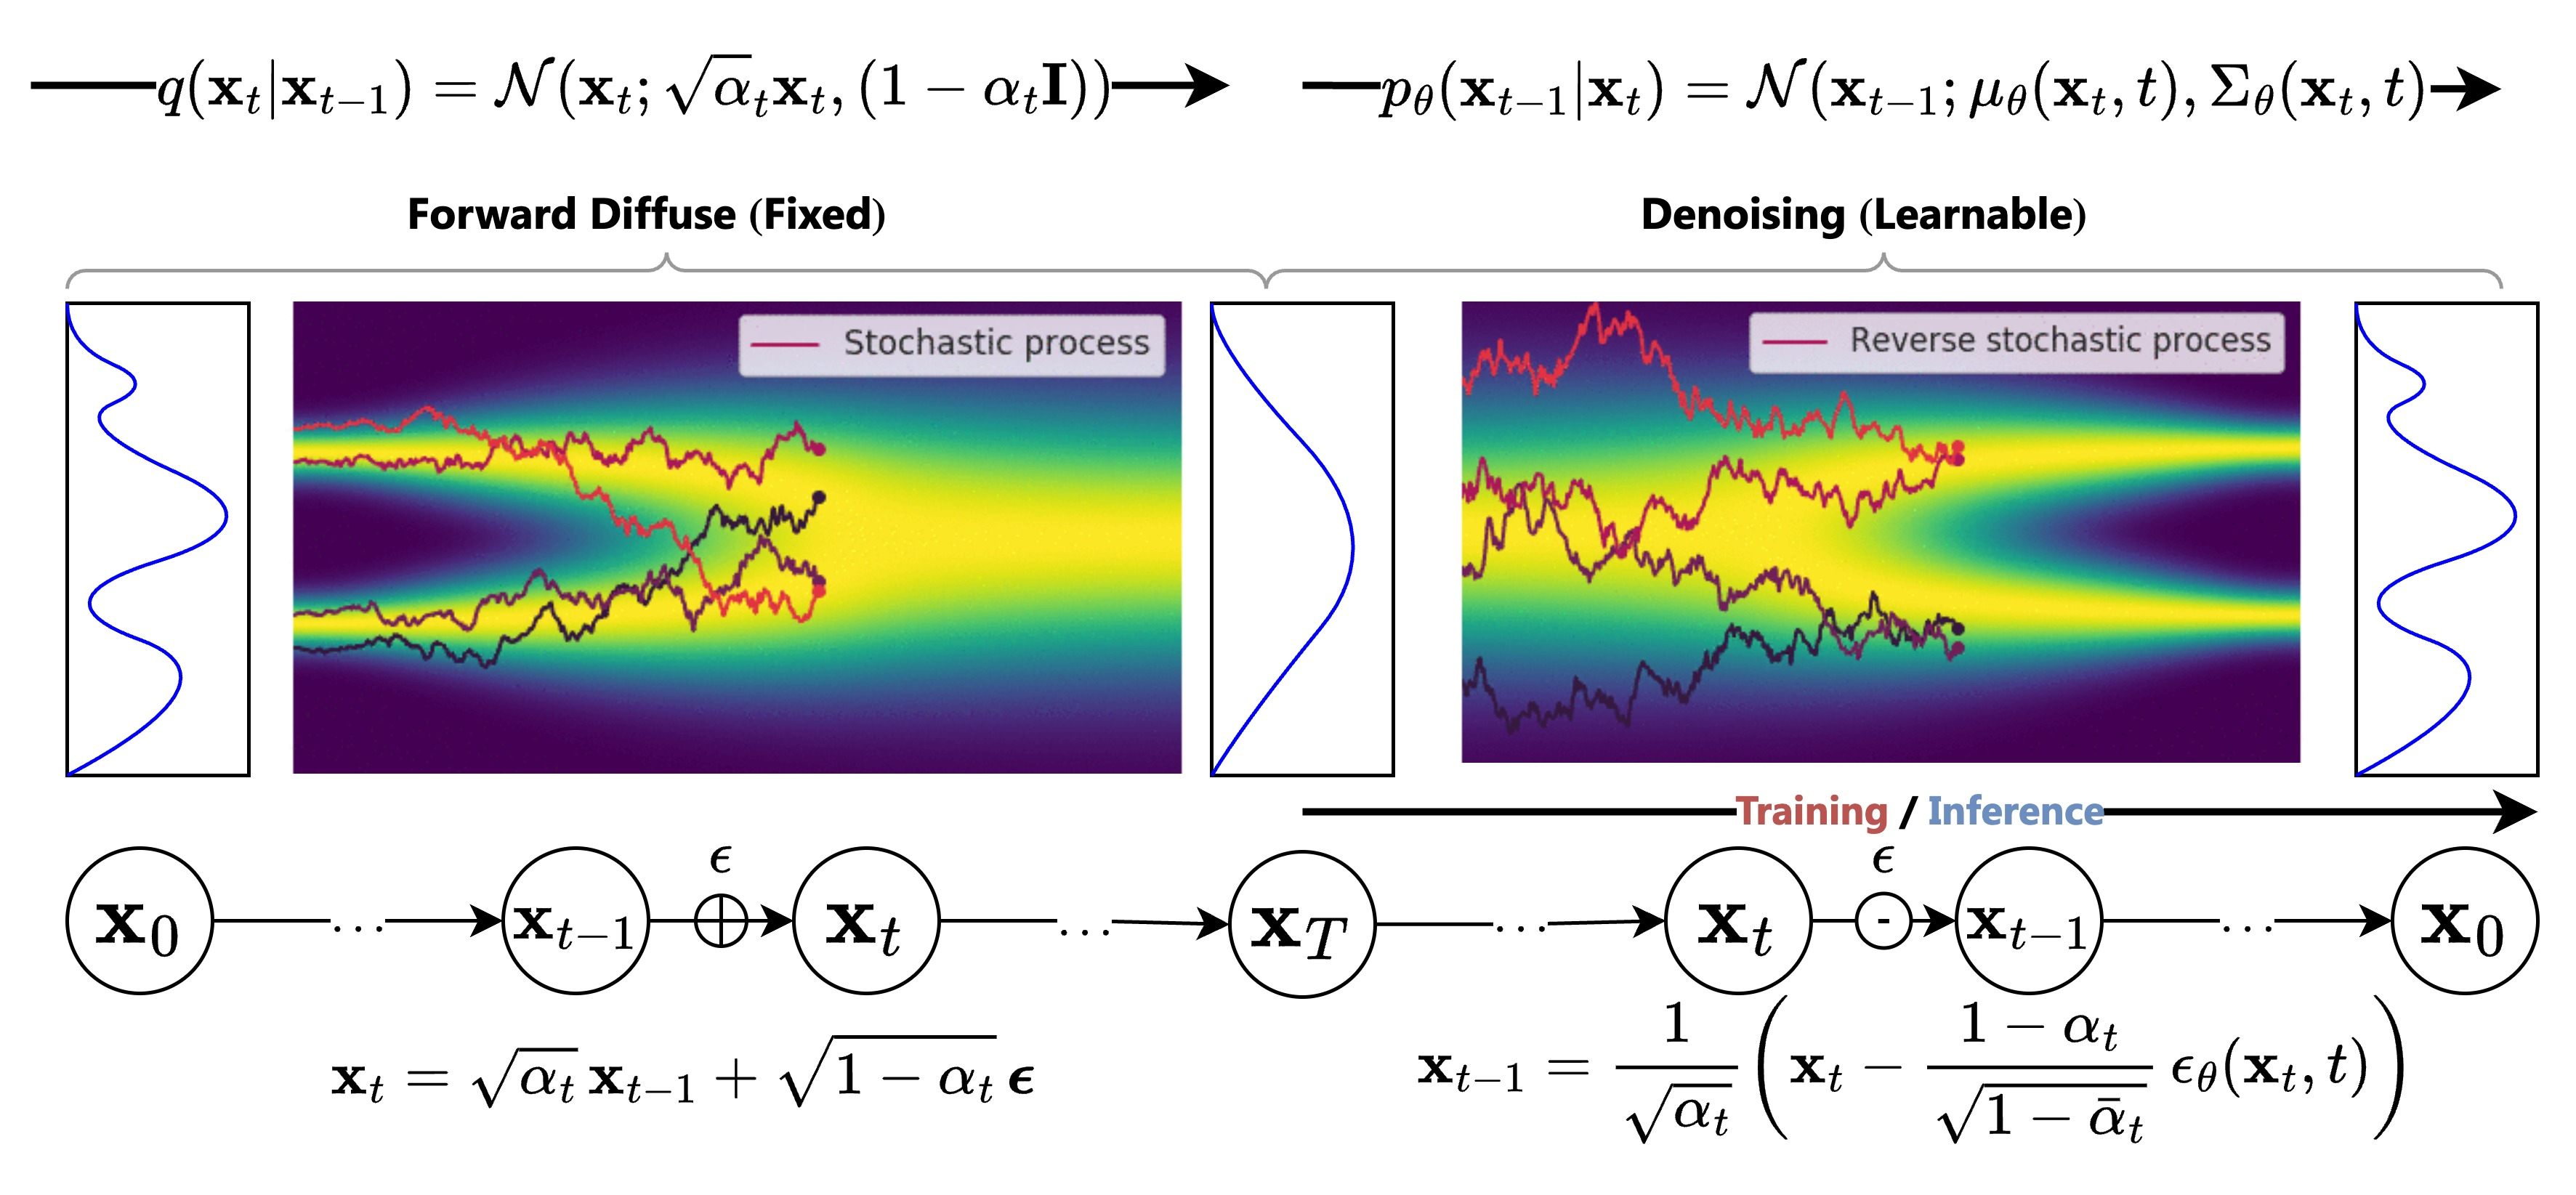
\includegraphics[width=\textwidth]{PQ}
%	\end{figure}
%	
%	\begin{itemize}
%		\item $q (\mathbf{x}_{t} | \mathbf{x}_{t-1}) = \mathcal{N}(\mathbf{x}_t; \sqrt{\alpha}_t \mathbf{x}_t, (1 - \alpha_t \mathbf{I}))$
%		\item $p_\theta (\mathbf{x}_{t-1} | \mathbf{x}_{t}) = \mathcal{N}(\mathbf{x}_{t-1}; \mu_\theta{(\mathbf{x}_t, t)}, {\Sigma}_{\theta} {  (\mathbf{x}_t, t ) }$
%	\end{itemize}
%	%	$q(\mathbf{x}_t \vert \mathbf{x}_0) = \mathcal{N}(\mathbf{x}_t; \sqrt{\bar{\alpha}_t} \mathbf{x}_0, (1 - \bar{\alpha}_t)\mathbf{I})$
%	%
%	%
%	%
%	%\begin{equation}
%	%	\mathbf{x}_{t-1}=\frac{1}{\sqrt{1- \beta_t}}\left(\bx_t-\sqrt{\beta_t} \cdot \epsilon_{\color{red}{\theta}}\left(\mathbf{x}_t, t\right)\right)+\color{red}{\beta_t \cdot \sigma_t \mathbf{z}} \color{black}{}
%	%\end{equation}
%	
%\end{frame}
%
%\begin{frame}{Vanilla Diffusion với $\epsilon$ Objective}
%	\begin{figure}
%		\centering
%		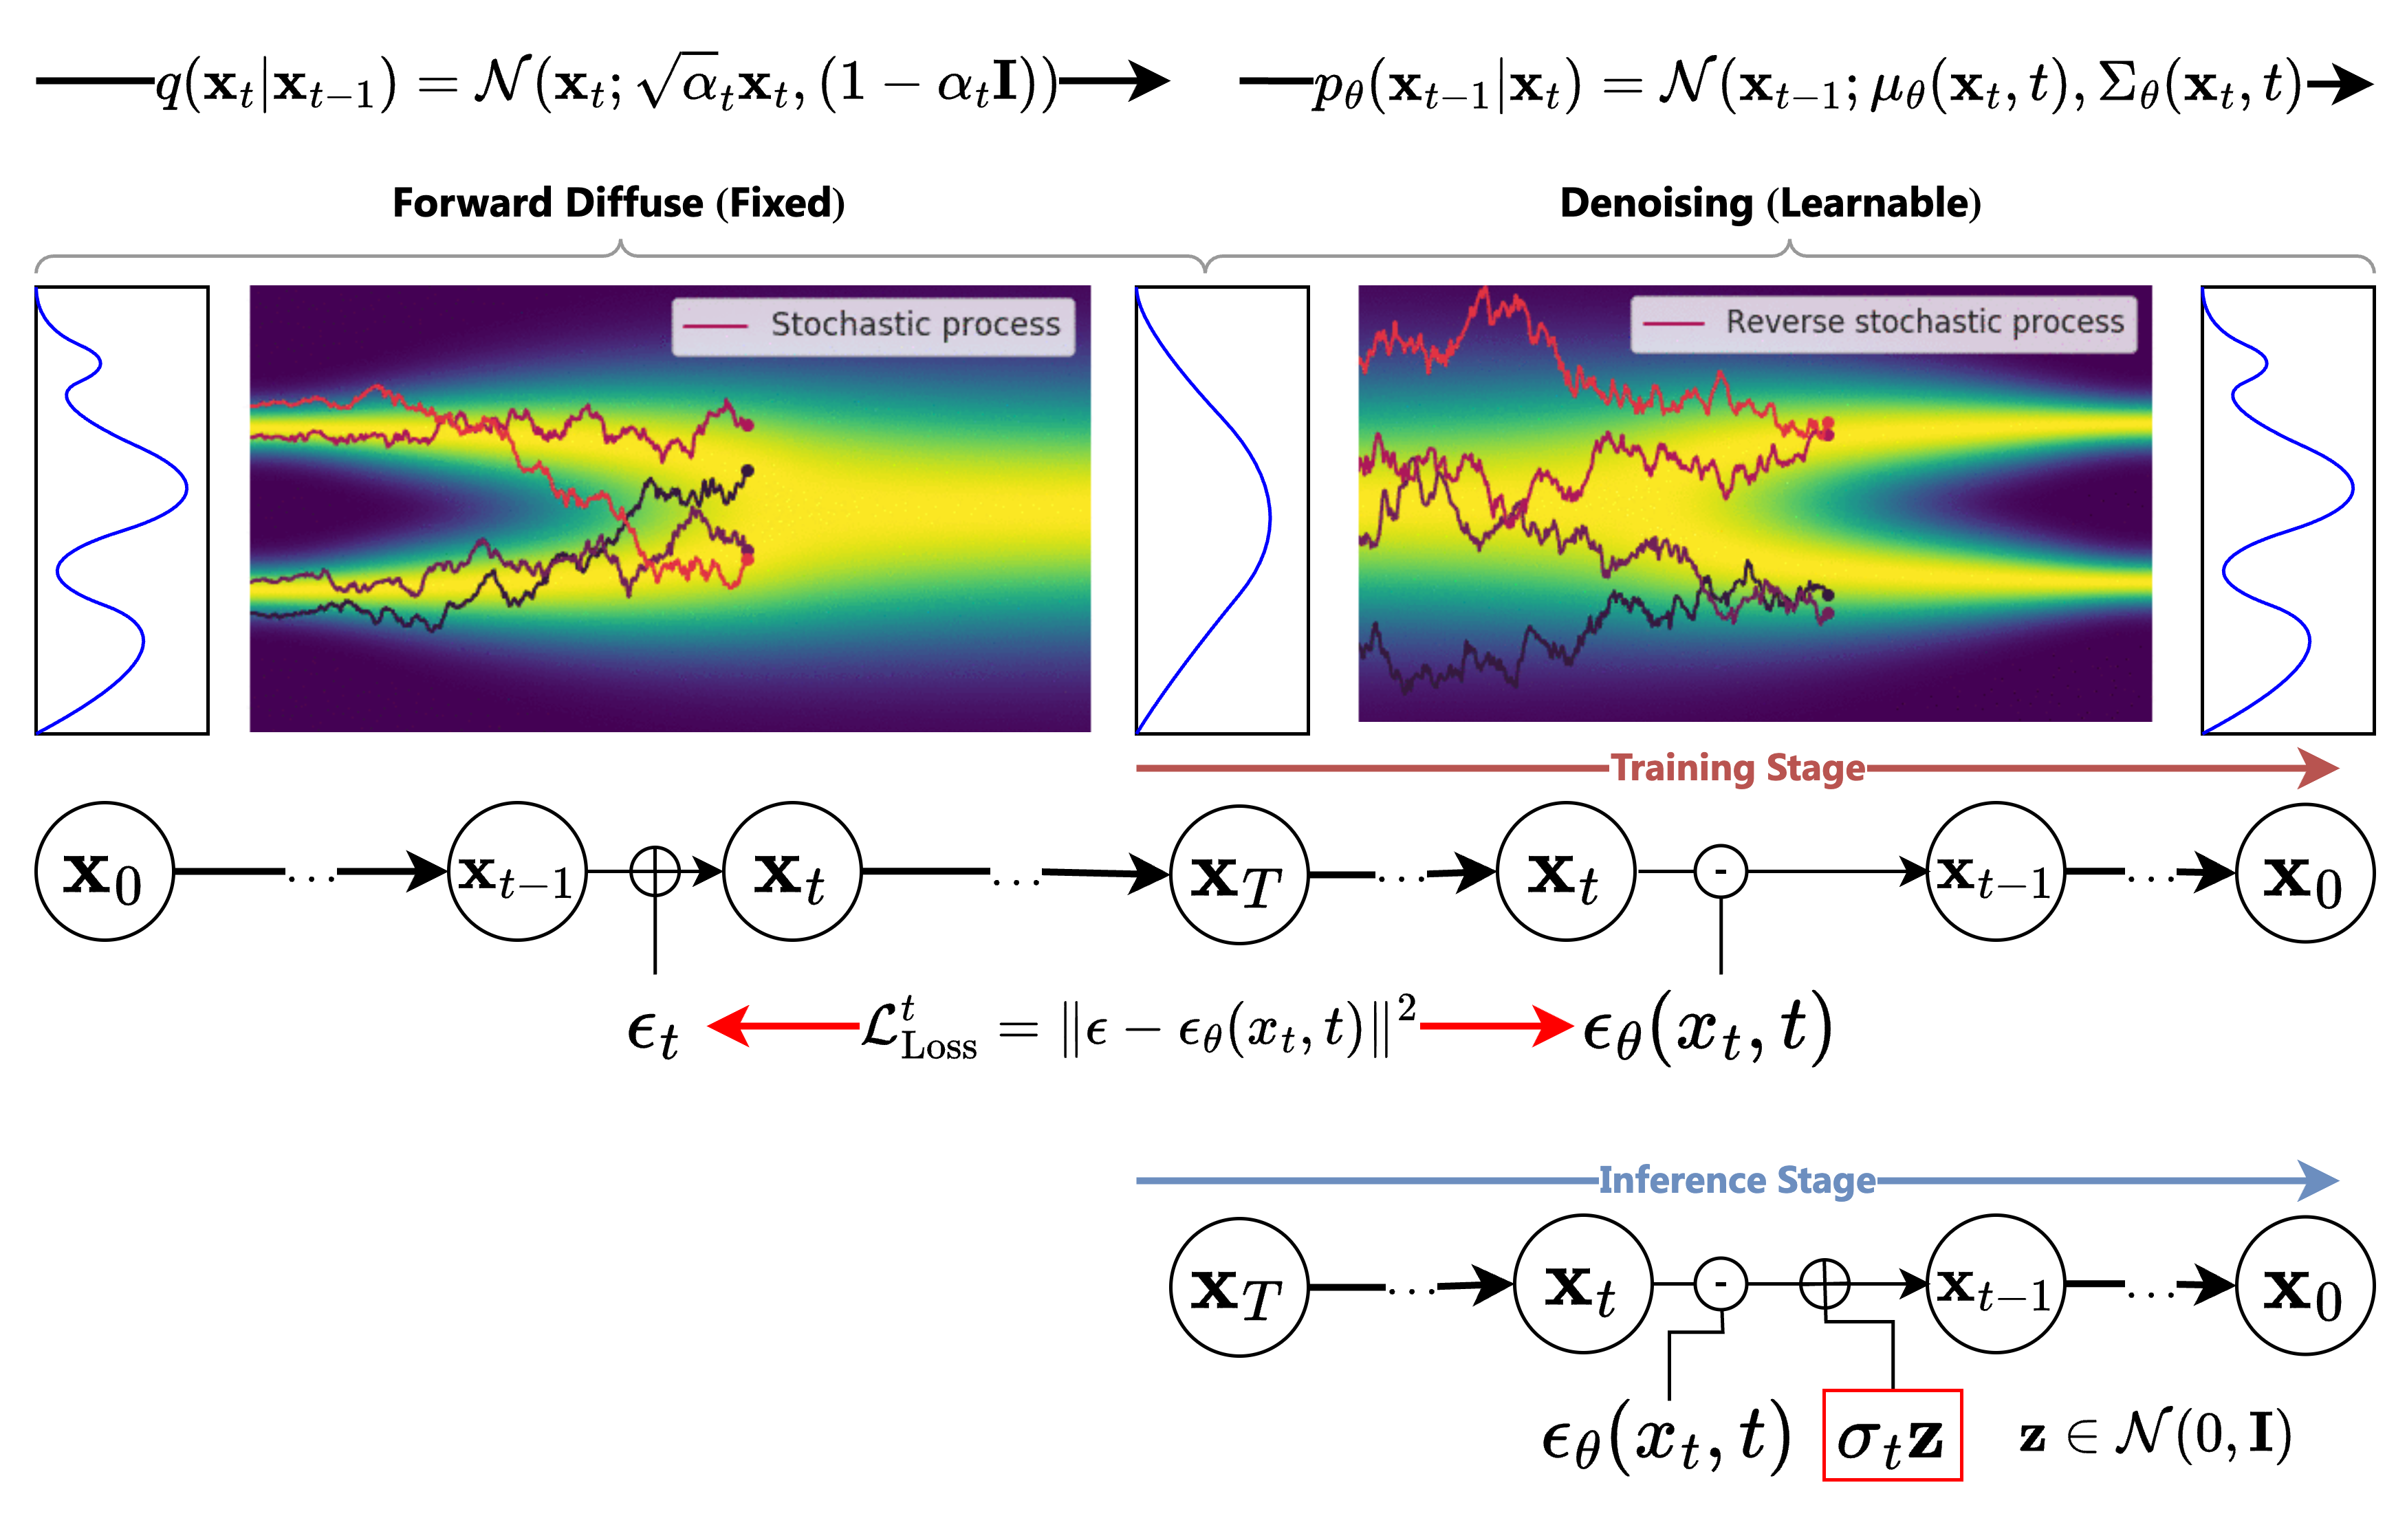
\includegraphics[width=0.95\textwidth]{TrainingAndSamplingStandard}
%	\end{figure}
%\end{frame}
%
%
%
%
%\begin{frame}{Quan hệ $\bx_{0}$, $\bx_t$ và $\bx_{t - 1}$}
%	
%	Ta có thể suy ra $\bx_t$ từ $\bx_0$ và ngược lại. Với $ \boldsymbol{\epsilon}_{t-1}, \boldsymbol{\epsilon}_{t-2}, \dots \sim \mathcal{N}(\mathbf{0}, \mathbf{I})$
%	%\begin{align*}
%	%	\mathbf{x}_t & = \sqrt{\alpha_t}\mathbf{x}_{t-1} + \sqrt{1 - \alpha_t} \boldsymbol{\epsilon}_{t-1} \\
%	%	& = \sqrt{\alpha_t \alpha_{t-1}} \mathbf{x}_{t-2} + \sqrt{1 - \alpha_t \alpha_{t-1}} \bar{\boldsymbol{\epsilon}}_{t-2} \\
%	%	& = \dots \\
%	%	& = \sqrt{\bar{\alpha}_t}\mathbf{x}_0 + \sqrt{1 - \bar{\alpha}_t}\boldsymbol{\epsilon}
%	%\end{align*}
%	\vspace{-10pt}
%	
%	\begin{figure}
%		\centering
%		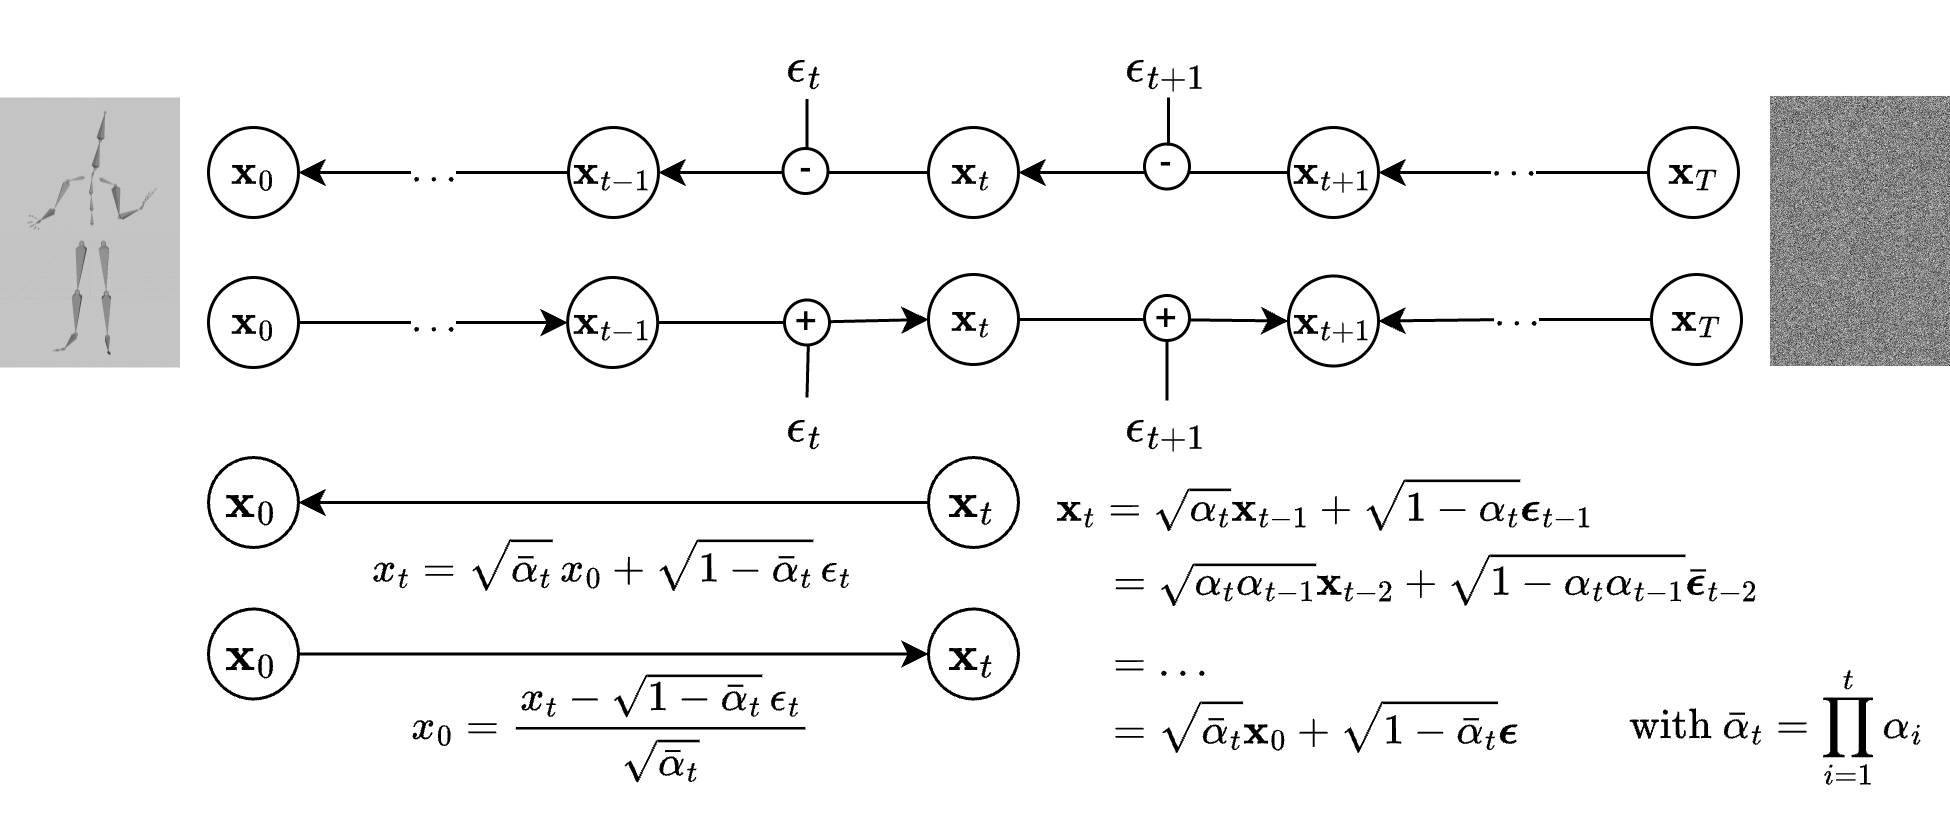
\includegraphics[width=\textwidth]{XRelation.png}
%	\end{figure}
%	%\vspace{-10pt}
%	%	\mathbf{x}_t = \sqrt{\bar{\alpha}_t}\mathbf{x}_0 + \sqrt{1 - \bar{\alpha}_t}\boldsymbol{\epsilon}
%	\begin{columns}
%		\begin{column}{0.5\textwidth}
%			\begin{itemize}
%				\item $\bar{\alpha}_1 > \dots > \bar{\alpha}_T$
%				\item Tổng hai nhiễu cũng là nhiễu:
%				\footnotesize
%				$$
%				\mathcal{N}(\mathbf{0}, \sigma_1^2\mathbf{I}) + 
%				\mathcal{N}(\mathbf{0}, \sigma_2^2\mathbf{I})
%				=\mathcal{N}(\mathbf{0}, (\sigma_1^2 + \sigma_2^2)\mathbf{I})
%				$$
%			\end{itemize}
%		\end{column}
%		\begin{column}{0.5\textwidth}
%			
%			\begin{figure}
%				\centering
%				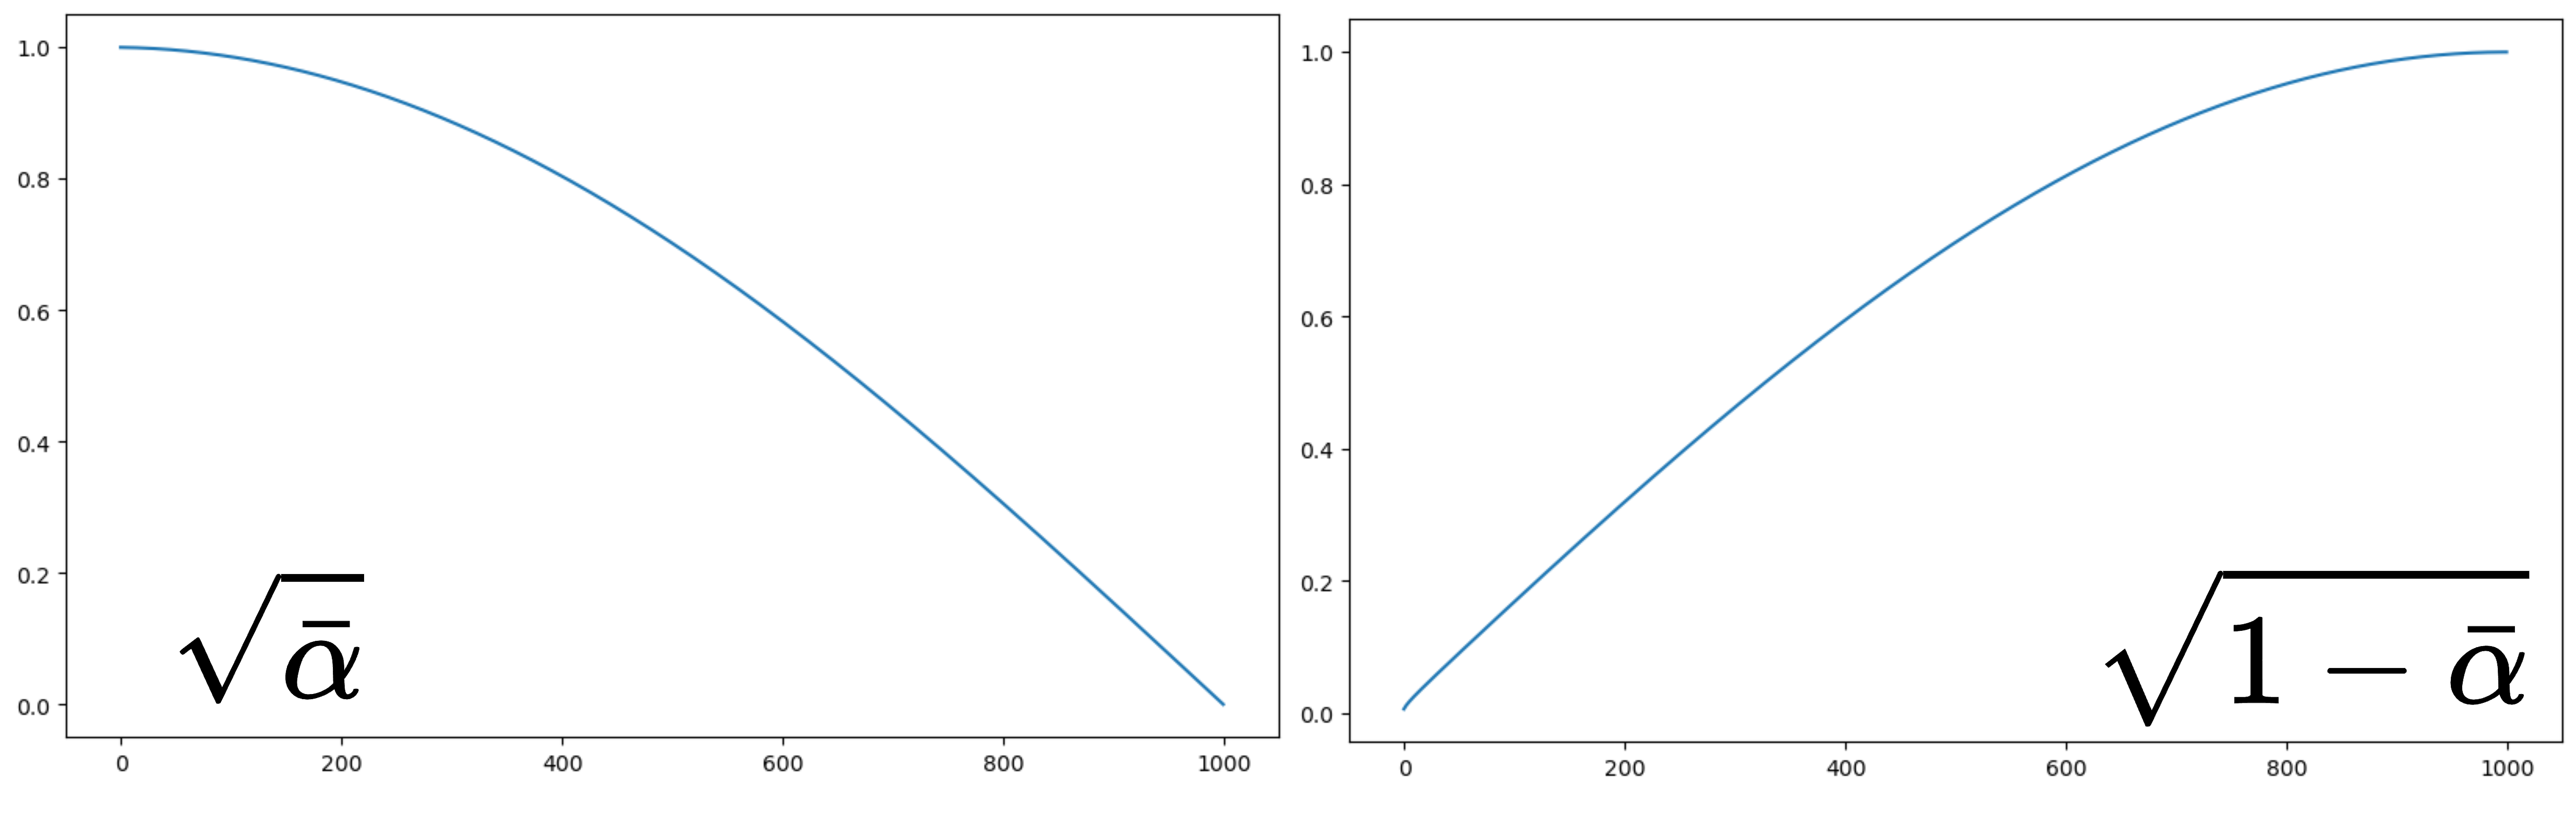
\includegraphics[width=\textwidth]{AlphaCumprod}
%			\end{figure}
%			
%			
%		\end{column}
%	\end{columns}
%	
%\end{frame}
%
%
%
%\begin{frame}{Cải tiến của DDIM \cite{song2020denoising} với $\mathbf{x}_0$ Objective (DALL E-2)}
%	Cải tiến của $\mathbf{x}_0$ objective so với $\epsilon$ objective
%	\begin{itemize}
%			\item Thay vì hàm $f_{\theta}(\bx_t, t)$ dự đoán nhiễu $\epsilon_t$ thì  $f_{\theta}(\bx_t, t)$ dự đoán $\bx_0$.
%			\item Sau khi có $\bx_0$ thì ta thêm nhiễu đã có từ trước (từ forward process) để được $\bx_{t-1}$
%	%		$$\tilde{\epsilon}\theta(x_t,t,c) = \epsilon\theta(x_t,t,\emptyset) + w[\epsilon_\theta(x_t,t,c) - \epsilon_\theta(x_t,t,\emptyset)]$$
%		\end{itemize} 
%	
%	\begin{figure}
%			\centering
%			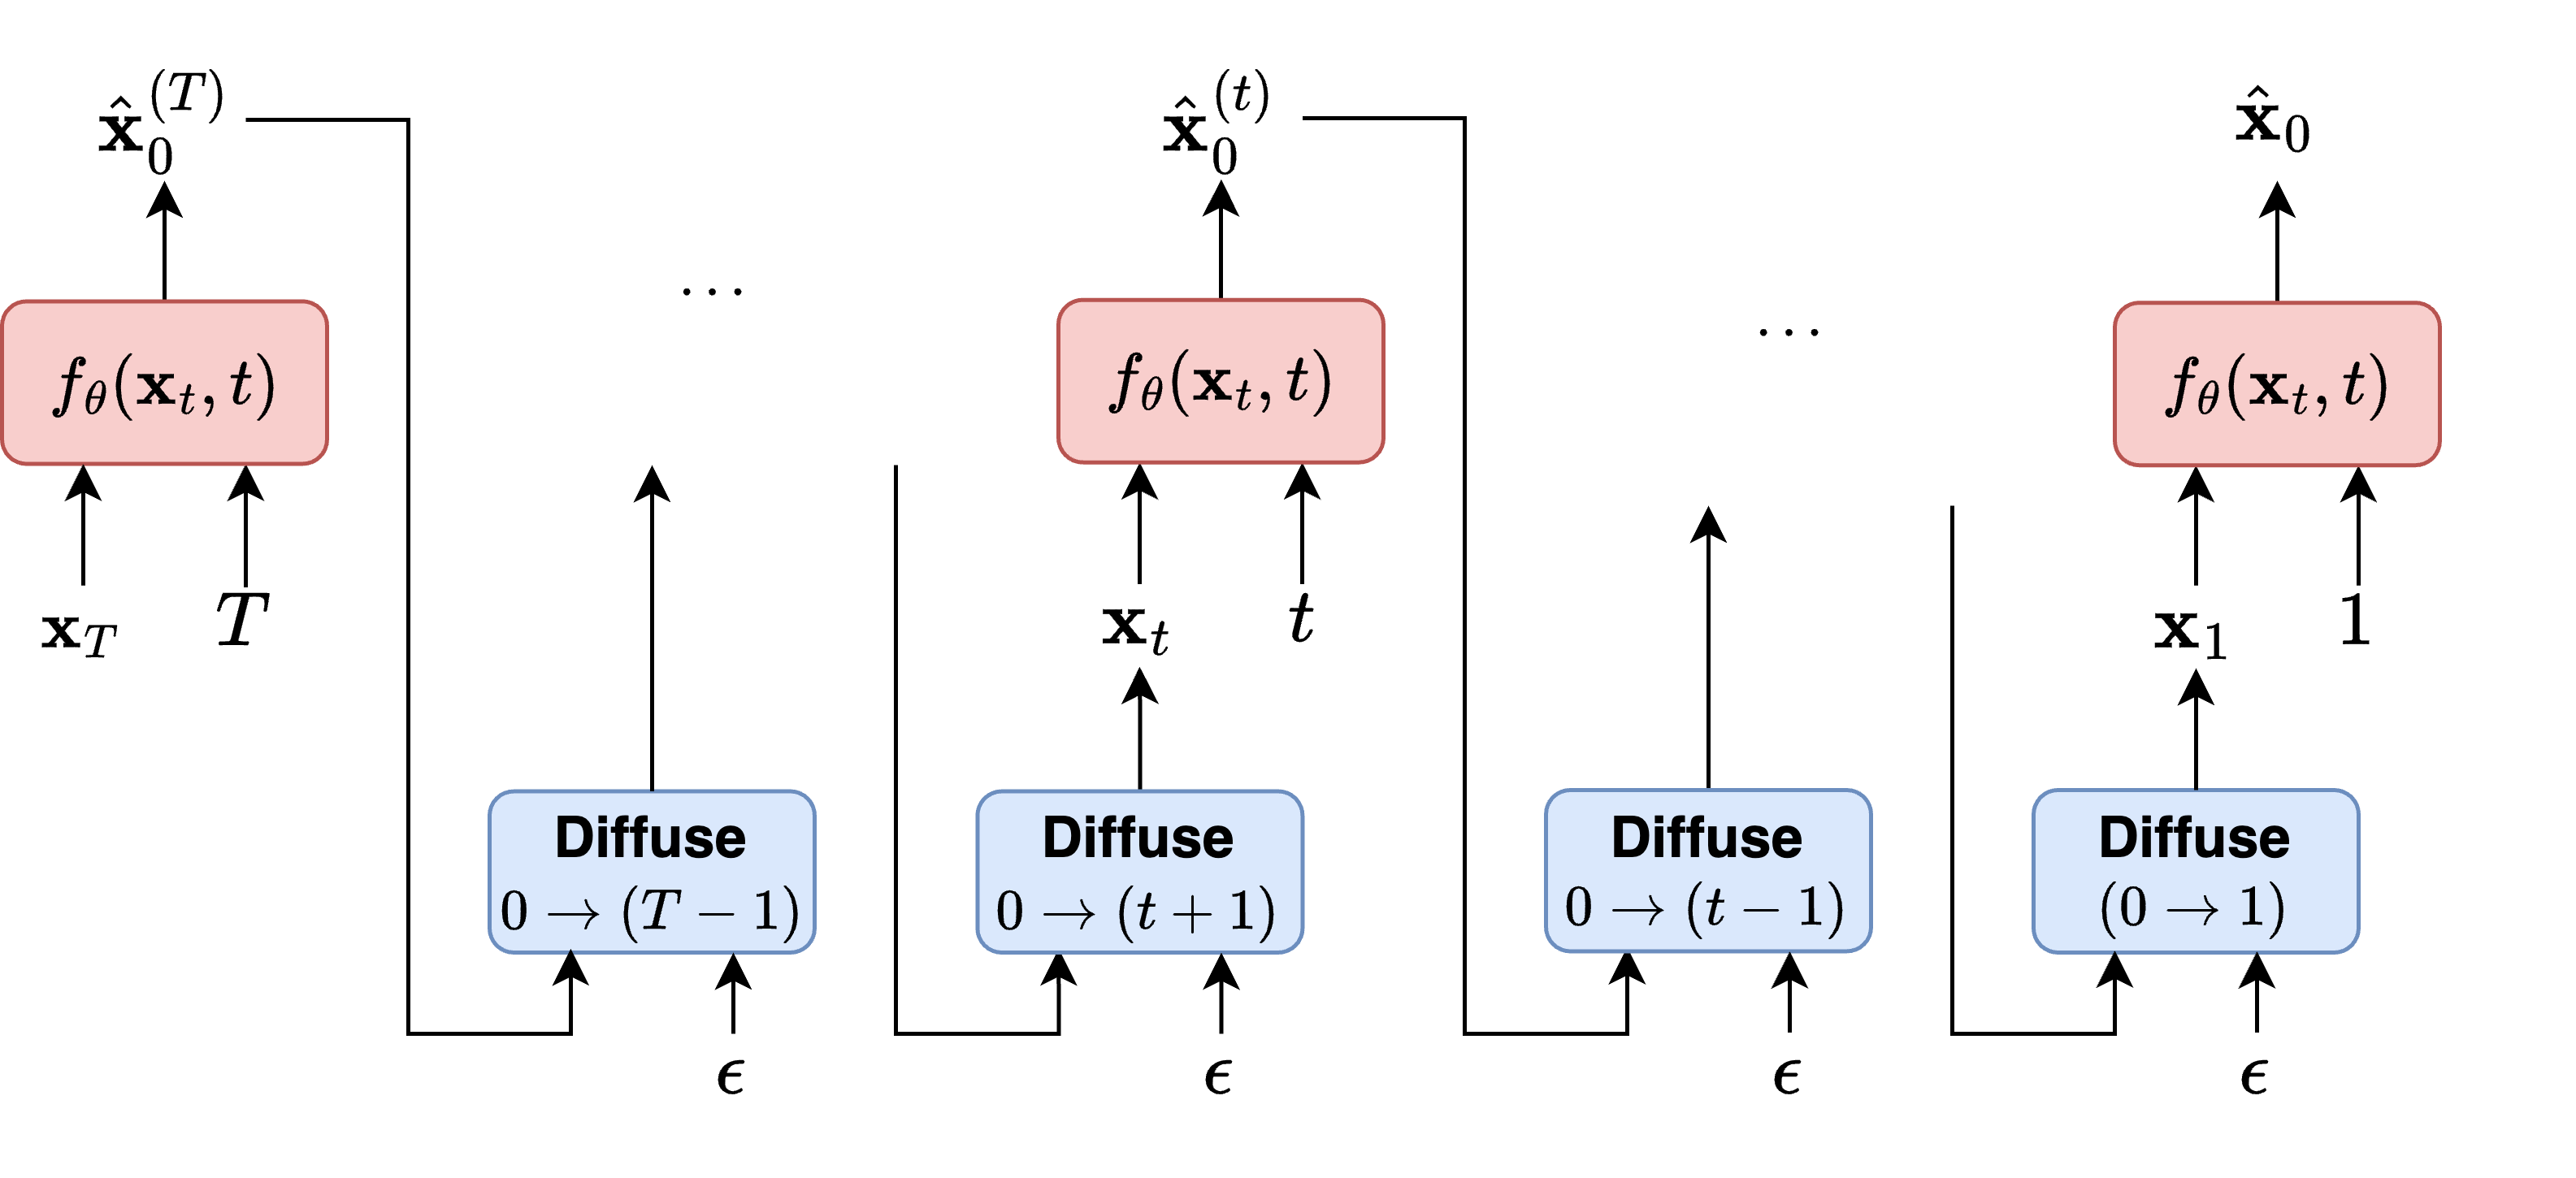
\includegraphics[width=0.95\linewidth]{SimpleX0Objective}
%		\end{figure}
%	
%\end{frame}
%
%\begin{frame}{Diffusion cho bài toán sinh cử chỉ}
%	
%	\begin{figure}
%		\centering
%		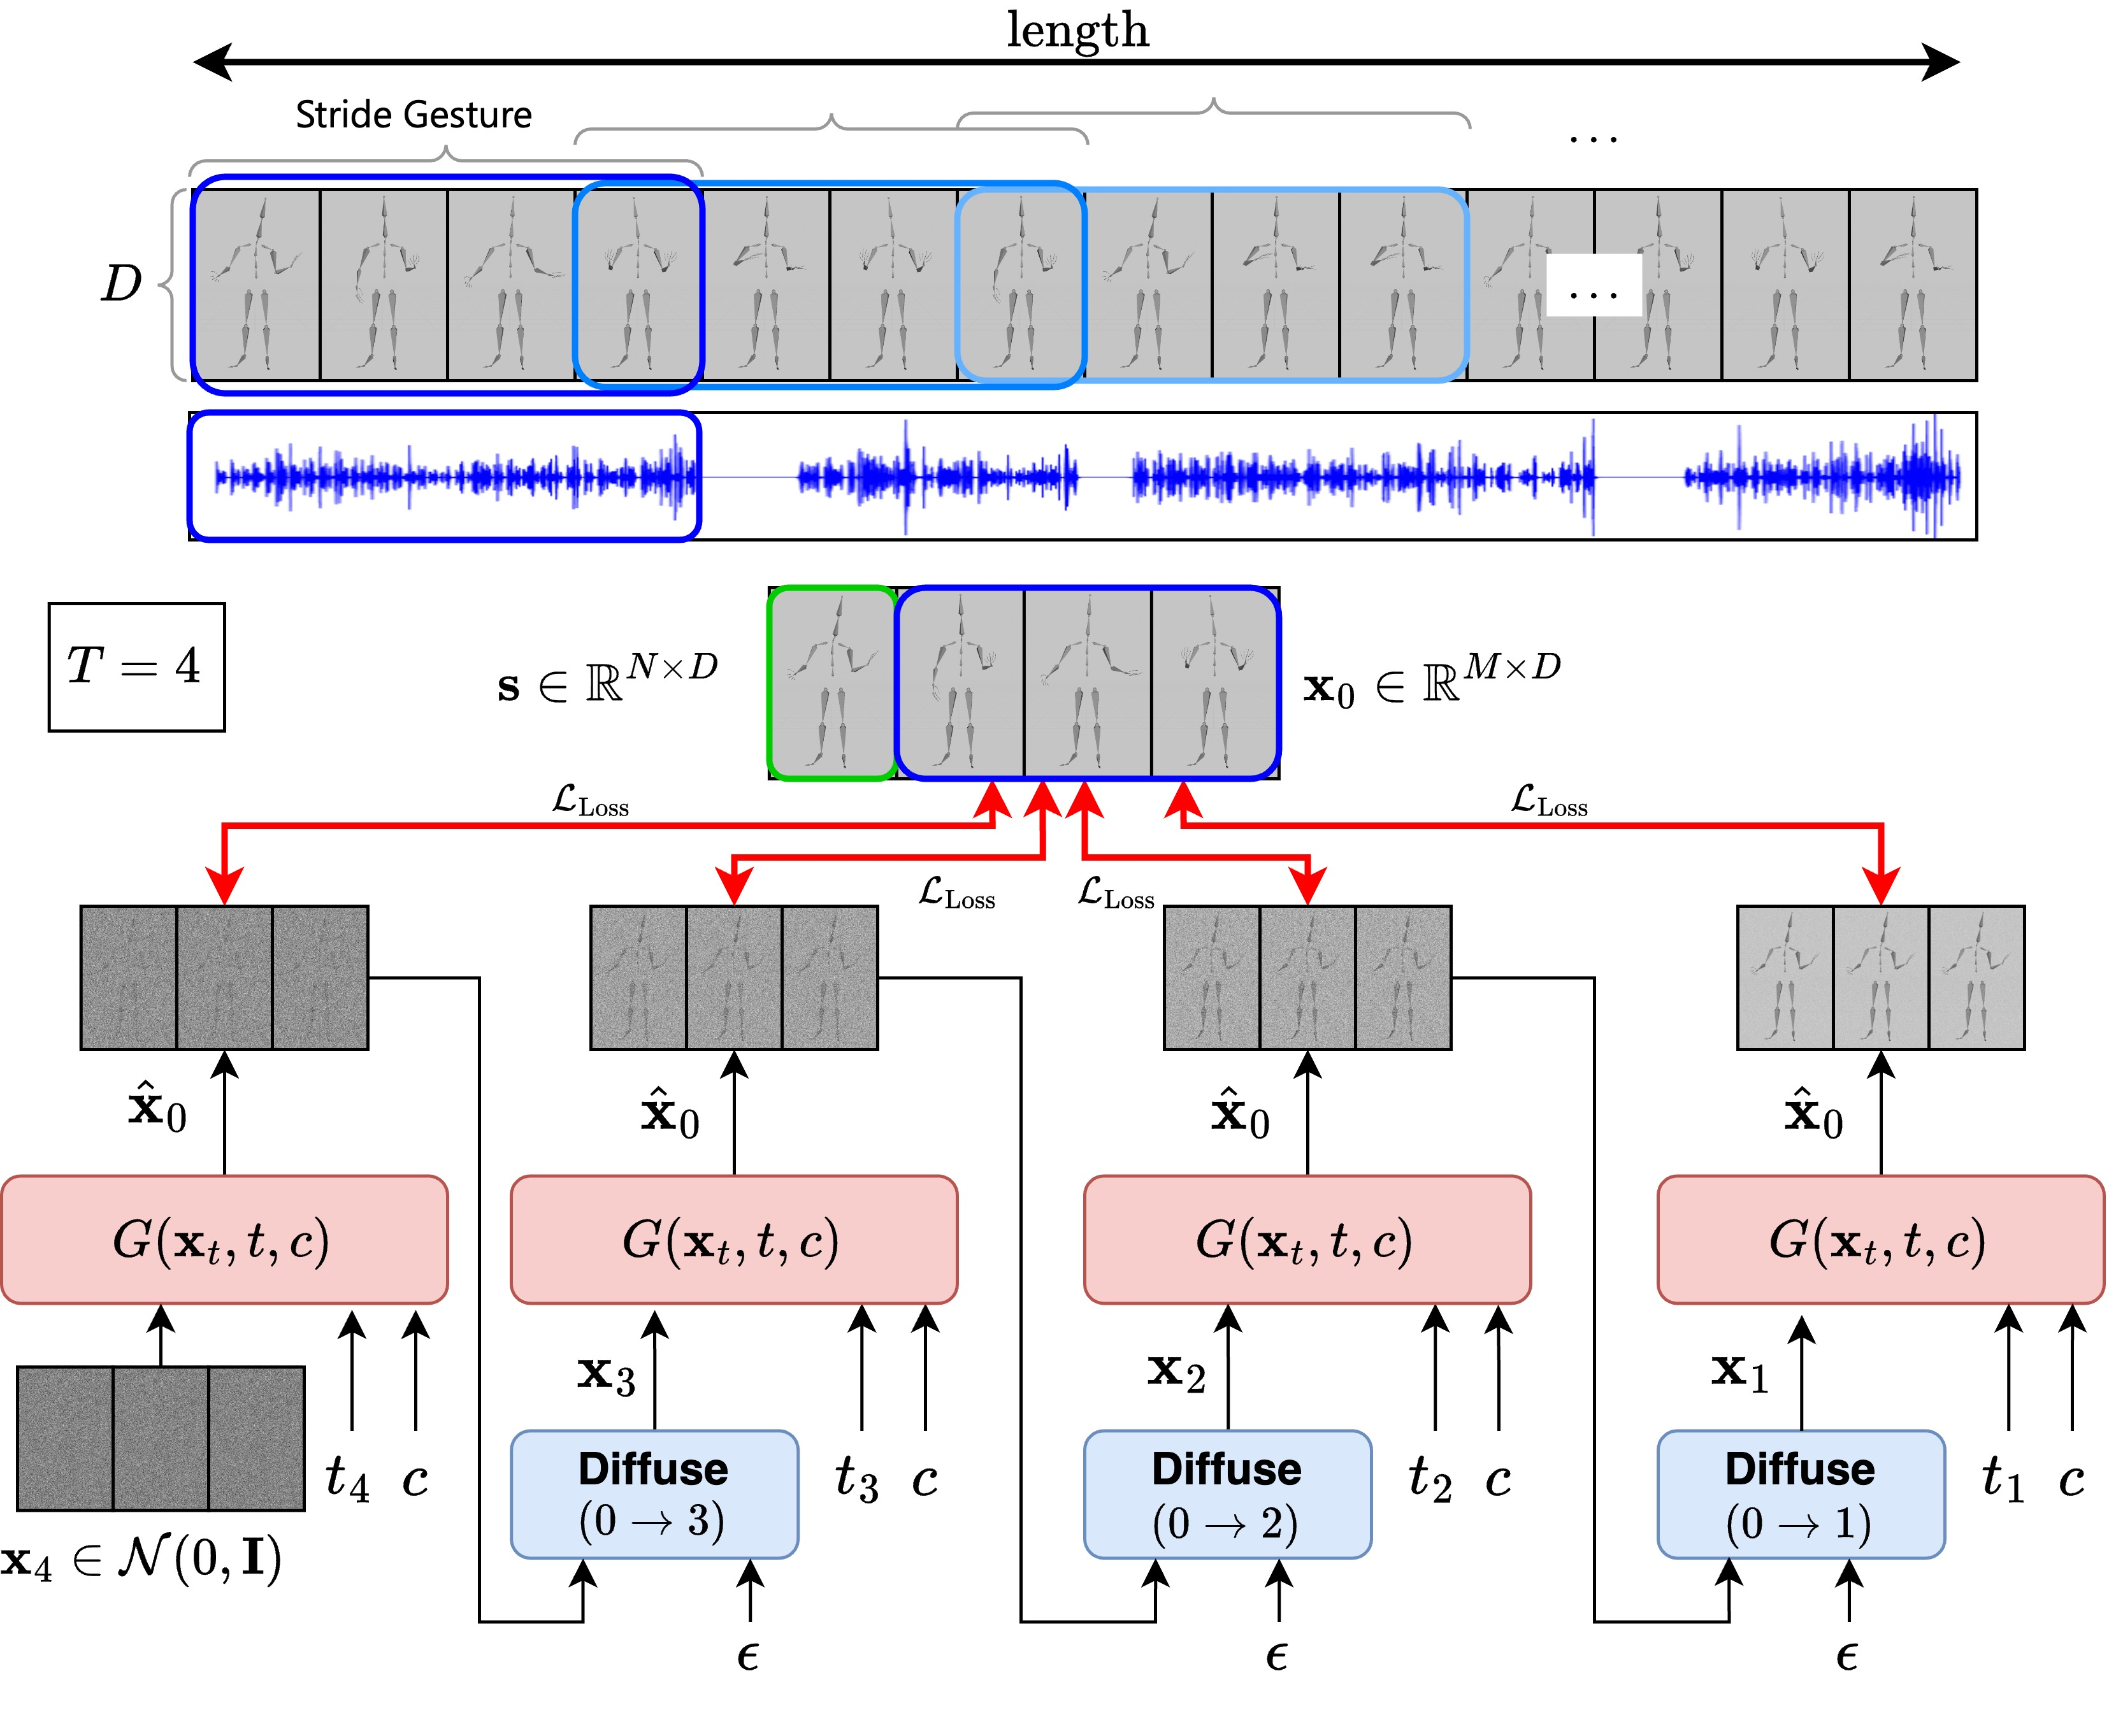
\includegraphics[width=0.9\linewidth]{OverviewArchitecture.jpg}
%	\end{figure}
%	
%\end{frame}
%
%\begin{frame}{Classifier-Free Guidance với $\mathbf{x}_0$ Objective}
%	\begin{figure}
%		\centering
%		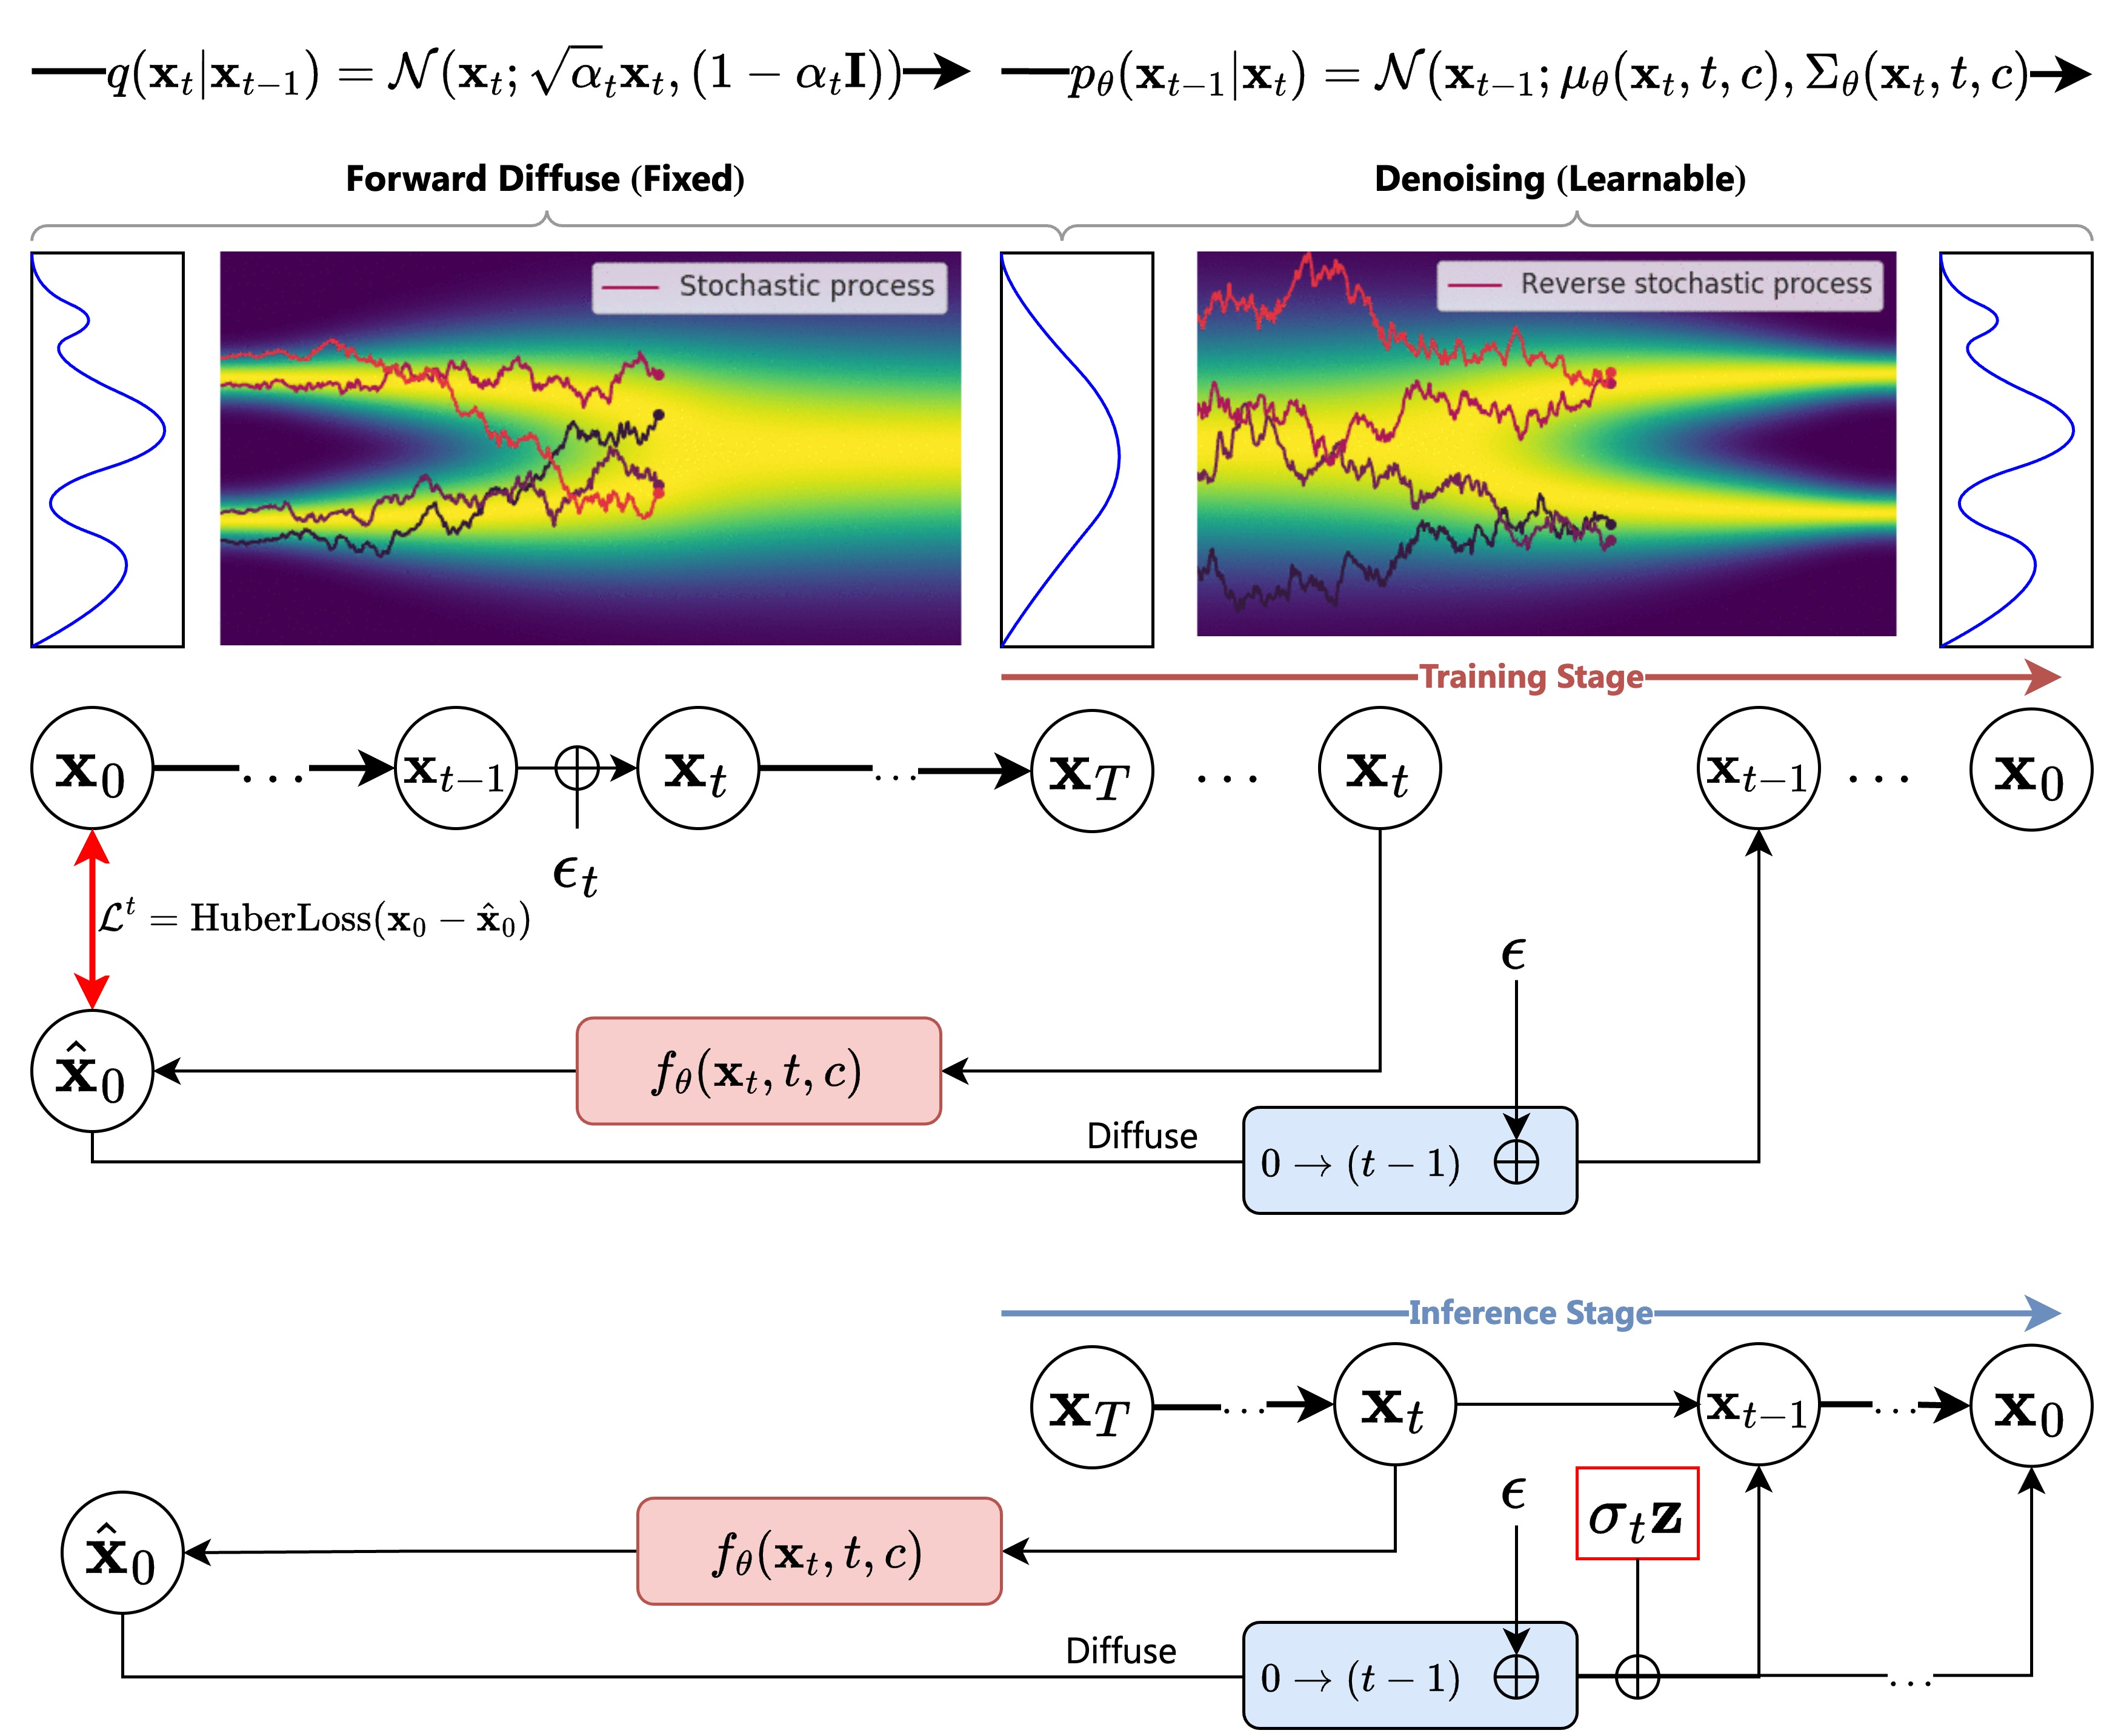
\includegraphics[width=0.9\linewidth]{TrainingAndSampling}
%	\end{figure}
%\end{frame}